\subsection{کنترل طبقه نرم}
برای کنترل نرمی طبقات نیاز به محاسبه سختی طبقات داریم! بحث های زیادی در رابطه با بدست آوردن سختی طبقات و نحوه بدست آوردن آن مطرح است. جناب دکتر اصغری یک یادداشت نسبتا مفصل در رابطه با روشهای بدست آوردن سختی دارند که توصیه میشود حتما مطالعه نمایید.

در نرم افزار سیویل تولز مجموعا ۳ روش برای محاسبه سختی پیاده سازی شده است که به ترتیب روش 2800، مودال و نیرو-تغییرمکان می باشد. کاربر با زدن آیکن مربوط به محاسبه سختی طبقات با پنجره ای مطابق شکل 
\ref{pic:stiffness_way_dialog}
روبرو میشود. پیش فرض نرم افزار روش 2800 می باشد، اگر به کانال تلگرام من مراجعه کنید مقایسه ای بین این ۳ روش انجام دادم (البته خیلی محدود) و به نظر میرسد که روش استاندارد 2800 از دو روش دیگر منطقی تر باشد.

\textcolor{red}{برای محاسبه سختی طبقات در روشهای 2800 و مودال باید کاربر از طریق منوی \lr{Analyze -> Set Load Cases to Run} گزینه \lr{Calculate Diaphragm Centers of Rigidity} را فعال کند (شکل \ref{pic:stiffness_way_dialog}) }

\textcolor{red}{در روش نیرو یا همان روش سوم کاربر باید زلزله های بدون خروج از مرکزیت در دو راستا تعریف کند، مثلا $EX, EY$، نام این بارها مهم نیست.}

\begin{figure}[H]
    \centering
    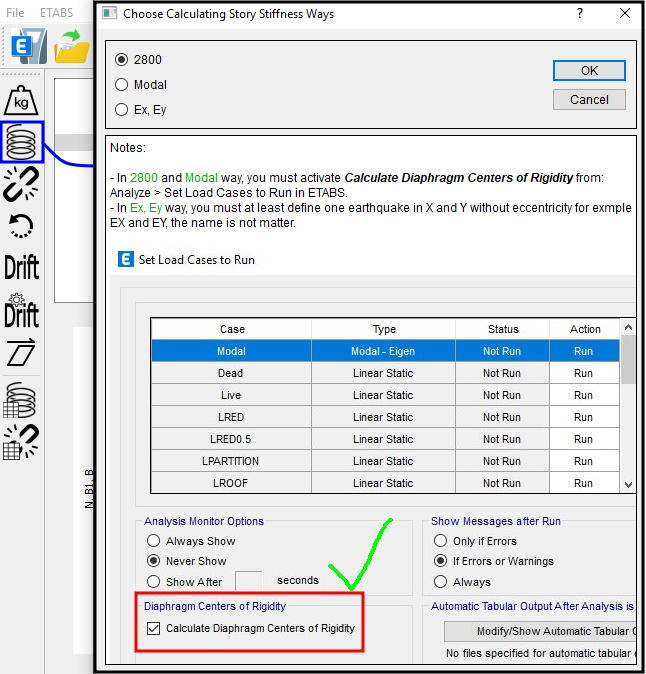
\includegraphics[scale=0.7]{figures/stiffness_dialog}
    \caption{پنجره انتخاب روش محاسبه سختی طبقات}
    \label{pic:stiffness_way_dialog}
\end{figure}

نرم افزار دو معیار سختی مطابق با شکل 
\ref{pic:stiffness_low}
را چک کرده و نتایج را به صورت جدول با رنگ بندی همانند جدول شکل \ref{pic:stiffness_2800} مشخص میکند:

\begin{figure}[H]
    \centering
    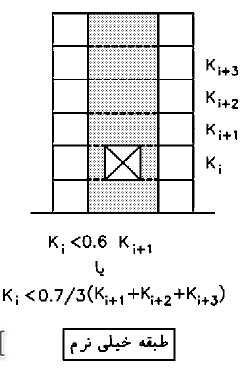
\includegraphics[scale=0.7]{figures/stiffness3}
    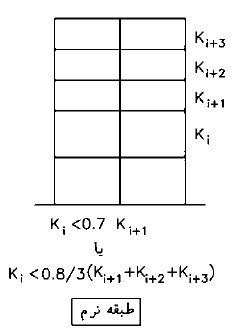
\includegraphics[scale=0.7]{figures/stiffness2}
    \caption{معیارهای کنترل سختی طبقات}
    \label{pic:stiffness_low}
\end{figure}

\subsubsection{روش استاندارد 2800}
در این روش نرم افزار به تعداد طبقات سازه، کپی از مدل اصلی میسازد. سپس در هر فایل،‌ با توجه به اینکه سختی کدام طبقه را میخواهد محاسبه کند، مراحل زیر را  برای هر فایل انجام میدهد:
\begin{itemize}
    \item مطابق شکل \ref{pic:tie_below_story_nodes} گره های طبقات پایینتر را در راستای $ x, y$ می بندد.
    \item سپس مرکز سختی طبقه را محاسبه میکند.
    \item  یک گره در مرکز سختی ایجاد میکند.
    \item این گره را به دیافراگم طبقه متصل میکند.
    \item مطابق شکل \ref{pic:stiffness_load} نیروی ۱۰۰۰ کیلوگرم در راستای $ x, y$ به این نقطه وارد میکند.
    \item سازه را تحلیل میکند و جابجایی نقاط در راستای $ x, y$ را میخواند.
    \item سپس با تقسیم نیرو به جابجایی سختی در راستای $ x, y$ را محاسبه میکند.
    \item این کار برای تمام طبقات صورت میگیرد و فایل های ساخته شده در محل فایل اصلی ذخیره میگردند تا بعدا بتوان به همراه فایل اصلی به نظام مهندسی ارسال کرد.
    \item  در نهایت این کنترل ها در  یک  جدول به صورت شکل \ref{pic:stiffness_2800} نمایش داده میشوند. فایل نتایج هم در محل فایل اصلی ذخیره میشود.
\end{itemize}

در شکل \ref{pic:stiffness_2800} مشاهده میشود که با توجه به ارتفاع زیاد طبقه همکف این طبقه به عنوان طبقه نرم مشخص شده است. رنگ زرد به معنای طبقه نرم و رنگ قرمز طبقه خیلی نرم می باشد.

\begin{figure}[H]
    \centering
    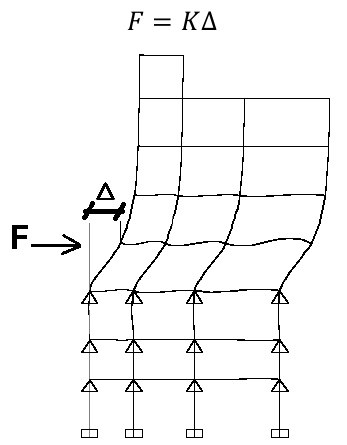
\includegraphics[scale=0.8]{figures/stiffness1}
    \caption{بستن گره های طبقات پایینی در راستای $x, y$ }
    \label{pic:tie_below_story_nodes}
\end{figure}

\begin{figure}[H]
    \centering
    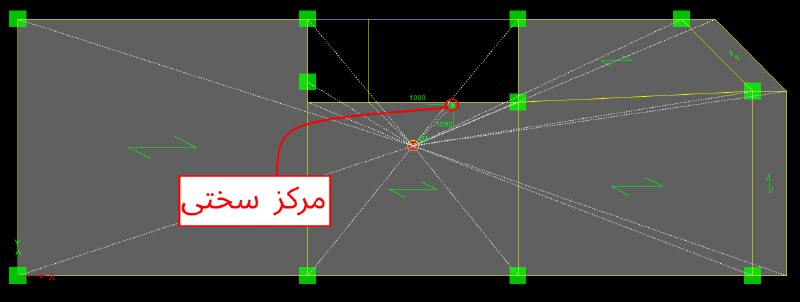
\includegraphics[scale=0.7]{figures/stiffness_load_in_center_of_rigidity}
    \caption{اعمال نیروی ۱۰۰۰ کیلوگرم در مرکز سختی طبقه}
    \label{pic:stiffness_load}
\end{figure}

\begin{figure}[H]
    \centering
    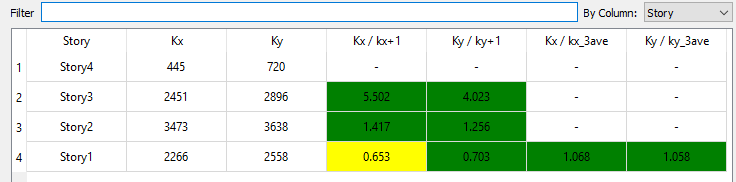
\includegraphics[scale=0.7]{figures/stiffness_2800}
    \caption{جدول نمایش سختی طبقات و کنترل نرمی طبقات}
    \label{pic:stiffness_2800}
\end{figure}

\subsubsection{روش مودال}
در این روش با استفاده از خصوصیات ذاتی سازه سختی طبقات بدست می آید و نیرویی به سازه وارد نمیشود. 
مراحل کار نرم افزار برای بدست آوردن سختی طبقات به ترتیب زیر است:
\begin{itemize}
    \item یک کپی از فایل اصلی گرفته میشود.
    \item یک نقطه در مرکز سختی تمام طبقات ایجاد میشود.
    \item  هر نقطه به دیافراگم مربوط به همان سقف متصل میشود.
    \item  آنالیز مودال انجام میشود.
    \item  فرکانس های جهت $x, y$ بدست میاید.
    \item  جرم طبقات از مدل استخراج میشود.
    \item شکل مودهای اصلی در راستای $x, y$ بدست می آید.
    \item سختی طبقات مطابق با فرمول \ref{eq:modal_stiffness} در دو راستای مجزا بدست می آید.
\end{itemize}

\begin{equation} \label{eq:modal_stiffness}
    \begin{split}
        K_1 & = \frac{\omega^2 \sum_{i=1}^{n}(m_i \phi_i)}{\phi_1} \\
        K_{n-1} & = \frac{\omega^2 \sum_{i=n-1}^{n}(m_i \phi_i)}{\phi_{n-1} - \phi_{n-2}} \\
        K_n & = \frac{\omega^2 m_n \phi_n}{\phi_n - \phi_{n-1}}
    \end{split}
\end{equation}

\subsubsection{روش نیرو-تغییرمکان}
در این روش از خروجی نرم افزار ایتبز برای محاسبه سختی استفاده میشود. بدین صورت که زلزله های بدون خروج از مرکزیت، به طور مثال 
$EX, EY$
 تشخیص داده میشود و سپس با آنالیز سازه نتایج سختی طبقات استخراج میشود.
در این روش برخی از کاربران نیروی زلزله را به خرپشته اعمال نمیکنند که سختی این طبقه برابر صفر گزارش میشود.
